\documentclass[usenames,dvipsnames,10pt]{beamer} % beamer is the document class for presentation slides

% needed for some examples
\usepackage[french]{babel}
\usepackage[autolanguage]{numprint}
\usepackage{amsmath} % even more advanced math
\usepackage{esint} % more integral (math) symbols

% languages typesetting rules
\usepackage{polyglossia} % handle multiple languages typesetting rules
\setdefaultlanguage{french} % this presentation is in french
\setotherlanguages{english,greek} % this presentation sometimes uses english and greek texts
\newfontfamily\greekfont[Script=Greek]{Linux Libertine O} % we need a special font for greek text
\newfontfamily\greekfontsf[Script=Greek]{Linux Libertine O} % same, but sans serif

% links configuration
\usepackage{hyperref} % commands such as \href, \url, etc.
\hypersetup{
    colorlinks=true,
    linkcolor=,
    urlcolor=NavyBlue,
    citecolor=Green
}

% bibliography configuration
\usepackage[backref=true]{biblatex} % bibliography handling
\newcommand{\titlecite}[1] {
    % Insert the (short) title of the citation, and a reference to it
    \citetitle{#1}\cite{#1}
}

% Configuration to nicely display code examples
\usepackage[skins,minted]{tcolorbox} % fancy colored boxes
\tcbset{ % configure the boxes style
    enhanced, % fancier boxes
    drop shadow,
    overlay={%
        % Add a small darker column to the left of the boxes to receive line numbers
        \begin{tcbclipinterior}
            \fill[gray!25] (frame.south west) rectangle ([xshift=4mm]frame.north west);
        \end{tcbclipinterior}
    }
}
\usemintedstyle[latex]{autumn}
\newmintedfile[texinput]{latex}{ % Shorthand for displaying latex code from file
    linenos, % display line numbers
    numbersep=2mm, % by default line numbers are too far on the left and leave the color box, make them closer
    fontsize=\footnotesize, % make the code smaller
    breaklines=true % break lines if they are too long
}
\newcommand{\texinputbox}[2]{
    % Display latex code through minted inside a color box
    \begin{tcolorbox}[title=#1,colframe=PineGreen]
        \selectlanguage{english}
        \texinput{#2}
    \end{tcolorbox}
}
\newcommand{\texexample}[5]{
    % Shorhand to display side by side a latex source file (minted) and its
    % rendering
    \begin{columns}
        \begin{column}{#4}
            \texinputbox{#2}{#1}
        \end{column}

        \begin{column}{#5}
            \begin{tcolorbox}[title=#3, overlay=]
                \input{#1}
            \end{tcolorbox}
        \end{column}
    \end{columns}
}
\definecolor{lightlightgray}{gray}{0.93}
\newmintinline[texinline]{latex}{bgcolor=lightlightgray} % Shorthand for \mintinline{latex}{…}
\newmintedfile[shellinput]{shell-session}{ % Shorthand for displaying shell sessions from file
    fontsize=\footnotesize, % make the code smaller
    breaklines=true, % break lines if they are too long
}
\newcommand{\shellinputbox}[2]{
    % Display shell session through minted inside a color box
    \begin{tcolorbox}[title=#1,overlay=,colframe=Violet]
        \selectlanguage{english}
        \shellinput{#2}
    \end{tcolorbox}
}

\usepackage{csquotes} % biblatex extensions for non-english languages
\usepackage{tipa} % International Phonetic Alphabet symbols and helpers
\usepackage{caption} % more control over captions
\usepackage{ccicons} % icons for Creative-Commons licenses
\usepackage{hologo} % tex and co. logos

% Beamer theme configuration
\usetheme{metropolis}
\metroset{sectionpage=none, subsectionpage=progressbar, progressbar=frametitle}
\setbeamertemplate{caption}[numbered] % Show figure number when using `\caption` instead of `\caption*`
\setbeamertemplate{footline}[page number] % Show the current page number in the bottom line of each slide

% define the \ipa command that switches to english typography rules before
% calling \textipa (which gets confused by french typography rules)
\newcommand{\ipa}[1] {
    \selectlanguage{english}
    \textipa{#1}
}

% Bibliography configuration
\bibliography{references}

% Meta information about this presentation
\title{Écriture de documents avec \LaTeX{}}
\subtitle{\texorpdfstring{\small{\emph{D'après une conférence de Didier Verna}\cite{latexDV}}}
                         {D'après une conférence de Didier Verna}}
\titlegraphic{\large{\href{https://creativecommons.org/licenses/by-sa/4.0/}{\ccbysa}}}
\institute[]{EPITA Strasbourg}
\author[Paul Hervot]{
    % The authors information appear in the first page of the document but also
    % in the pdf's metadata. A lot of stuff isn't allowed in the metadata
    % (links, line breaks, etc.) so we must define two alternatives, one for the
    % document page and one for the metadata, this is done with the
    % \texordpdfstring command
    \texorpdfstring
    { % Nicely formatted author information
        Paul Hervot\\
        \href{mailto:paul.hervot@epita.fr}{\nolinkurl{paul.hervot@epita.fr}}
    }{ % A simpler version for the pdf's metadata
        Paul Hervot
    }
}
\date{3 septembre 2019}

\begin{document}

\frame{\titlepage{}}

\section{Introduction}
\subsection{\TeX}
\begin{frame}{\TeX}
    \begin{description}
        \item[Nom :] symbolise les lettres \textgreek{τεχ}, abbréviation de \textgreek{τέχνη}
        \item[Objectif :] mise en forme typographique entièrement informatique
        \item[Création :] Donald Knuth, 1977-1989
        \item[Prononciation :] \ipa{[tEx]}
    \end{description}

    \begin{figure}[position]
        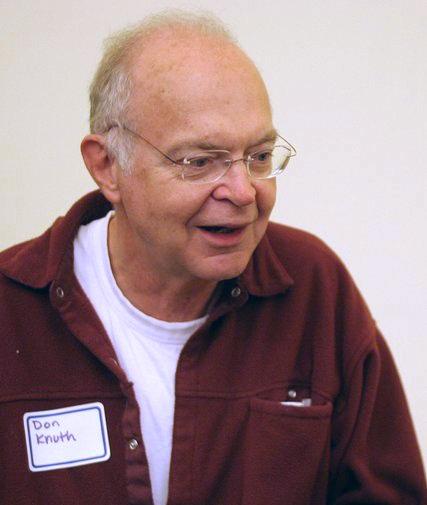
\includegraphics[height=0.5\textheight]{img/knuth}
        \caption*{Donald Knuth, en 2005\cite{knuthpic}}
    \end{figure}
\end{frame}

\subsection{\LaTeX}
\begin{frame}{\LaTeX}
    \begin{description}
        \item[Nom :] abbréviation de Lamport-\TeX
        \item[Objectif :] ensemble de macros (raccourcis) pour \TeX
        \item[Création :] Leslie Lamport, 1983
        \item[Prononciation :] \ipa{["lA:tEx]} ou \ipa{["leI:tEx]}
    \end{description}

    \begin{figure}[position]
        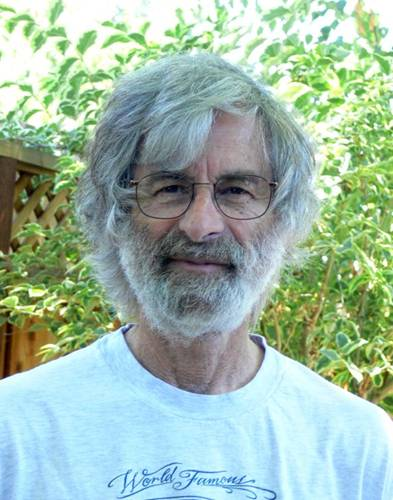
\includegraphics[height=0.5\textheight]{img/lamport}
        \caption*{Leslie Lamport, vers 2014}
    \end{figure}
\end{frame}

\begin{frame}{Intérêts aujourd'hui}
    \begin{itemize}
        \item édition mathématique ;
        \item gestion de bibliographie ;
        \item écriture sous forme de code source distribuable ;
        \item totalement libre, extensible ;
        \item très utilisé dans le milieu de la recherche.
    \end{itemize}
\end{frame}

\begin{frame}{Obtenir \LaTeX}
    \begin{description}
        \item[Multi-plateforme :] \href{http://tug.org/texlive/}{\TeX{}Live}.
            Standard \emph{de facto}, disponible dans toutes les distribution
            Linux.
        \item[Windows :] \href{https://miktex.org/}{\hologo{MiKTeX}}.
        \item[MacOS :] \href{https://www.tug.org/mactex/}{Mac\TeX}, basé sur \TeX{}Live.
        \item[En ligne :] \href{https://www.overleaf.com/}{Overleaf}, payant avec version d'essai.
    \end{description}

    \vspace{1cm}
    Il existe aussi de nombreux IDEs\footnote{Environnement de Développement
    Intégré} comme \href{https://www.xm1math.net/texmaker/}{\TeX{}Maker} et des
    plugins pour éditeurs comme \href{https://github.com/lervag/vimtex}{vimtex}.
    \LaTeX{} étant libre, il existe un très grand nombre d'outils autour.
\end{frame}

\section{Principes fondamentaux}
\subsection{Le langage}
\begin{frame}[fragile]{Organisation de la source d'un document \LaTeX}
    \texinputbox{article.tex}{examples/article-skeleton.tex}

    Anatomie d'une commande : \texinline{\nom[options]{arguments}}
\end{frame}

\begin{frame}[fragile]{Subtilités syntaxiques}
    \begin{itemize}
        \item Plusieurs caractères blancs $\Leftrightarrow$ un seul caractère blanc ;
        \item une ligne blanche $\Rightarrow$ changement de paragraphe ;
        \item caractères spéciaux à "échapper" par un \textbackslash{} :\\
            \texinline{\# \$ \% \^ \& \_ \{ \} \~}
        \item sauf pour \textbackslash{} qui s'écrira
            \texinline{\textbackslash{}} (car \texinline{\\}
            signifie "nouvelle ligne") ;
        \item commentaires : \texinline{%} jusqu'à la fin de la ligne
    \end{itemize}
\end{frame}

\begin{frame}[fragile]{Exemples}
    \texexample{examples/basics-syntax.tex}
               {exemple.tex}{exemple.pdf}
               {0.65\textwidth}{0.48\textwidth}

    \texexample{examples/basics-syntax-bis.tex}
               {}{}
               {0.65\textwidth}{0.48\textwidth}
\end{frame}

\subsection{Compilation}
\begin{frame}[fragile]{\hologo{XeTeX}}
    Il existe beaucoup d'outils en ligne de commande, \hologo{XeLaTeX} est le
    plus conseillé aujourd'hui.

    \shellinputbox{Compilation avec \hologo{XeLaTeX}}{examples/session-xelatex.session}

    \hologo{pdfLaTeX} est aussi très utilisé mais gère moins bien les accents et
    les polices modernes.
\end{frame}

\section{Fonctionnalités du langage}
\subsection{Configuration globale du document}
\begin{frame}[fragile]{Les classes de document}
    La classe d'un document est définie par la commande:

    \texinputbox{}{examples/documentclass-struct.tex}

    \begin{description}
        \item[Lettre :] \texinline{\documentclass[a4paper]{letter}}\\
            \textrightarrow{} \texinline{\signature{…}}, \texinline{\address{…}},
            etc…
        \item[Article :] \texinline{\documentclass{article}} \vspace{-5pt}
        \item[Rapport :] \texinline{\documentclass{report}} \vspace{-5pt}
        \item[Livres :] \texinline{\documentclass{book}}\\
            \textrightarrow{} \texinline{\title{…}}, \texinline{\author{…}}, etc…
        \item[Présentations :] \texinline{\documentclass{beamer}}\\
            \textrightarrow{} \texinline{\begin{frame}},
                \texinline{\usetheme{…}}, etc…
    \end{description}
\end{frame}

\begin{frame}[fragile]{Les paquets}
    Ajoutent des fonctionnalités (surtout des commandes) disponibles. Ils sont
    inclus avec:

    \texinputbox{}{examples/usepackage-struct.tex}

    \begin{description}
        \item[Liens cliquables:]
            \texinline{\usepackage[colorlinks=true]{hyperref}}\\
            \textrightarrow{} \texinline{\href{…}{…}}, \texinline{\url{…}}, etc…
        \item[Cadres colorés:] \texinline{\usepackage{tcolorbox}}\\
            \textrightarrow{} \texinline{\begin{tcolorbox}},
                \texinline{\tcbset{…}}, etc…
        \item[Coloration syntaxique:] \texinline{\usepackage{listings}}\\
            \textrightarrow{} \texinline{\begin{lstlisting}[language=Python]}\\
            (plus joli mais compliqué: \texinline{\usepackage{minted}})
    \end{description}

    Et \emph{beaucoup} d'autres.
\end{frame}

\begin{frame}[fragile]{Internationalisation (i18n)}
    Avec le paquet Babel:
    \texinputbox{}{examples/babel-fr.tex}

    Enjeux:
    \begin{itemize}
        \item respect automatique des règles de typographie (espaces devant les
        signes de ponctuation, césures, …);
        \item localisation des textes automatiques ("Table des matières",
        "Bibliographie", …);
        \item encodage et jeu de caractères du fichier source (voir aussi
        \texinline{\usepackage[utf8]{inputenc}}).
    \end{itemize}

    Il est aussi possible de gérer plusieurs langages dans un même document et
    de passer de l'un à l'autre avec des commandes (voir aussi
    \texinline{\usepackage{polyglossia}}).
\end{frame}

\begin{frame}[fragile]{Quelques éléments typographiques}
    \texexample{examples/typo-examples.tex}
               {exemple.tex}{exemple.pdf}
               {0.56\textwidth}{0.56\textwidth}
\end{frame}

\begin{frame}[fragile]{Exemple de typographie française\cite{imprimerie2002lexique}}
    \texexample{examples/typo-examples-fr.tex}
               {exemple.tex}{exemple.pdf}
               {0.57\textwidth}{0.55\textwidth}

    Note: \texinline{\nombre} vient du paquet "\texttt{numprint}" avec l'option
    "\texttt{autolanguage}" (\texinline{\usepackage[autolanguage]{numprint}}).
\end{frame}

\subsection{Table des matières}
\begin{frame}[fragile]{Exemple de ToC}
    \center
    \texinline{\section{…}}, \texinline{\subsection{…}},
    \texinline{\subsubsection{…}}

    \textrightarrow{} \texinline{\tableofcontents{}}
    \begin{columns}
        \begin{column}{0.5\textwidth}
            \begin{tcolorbox}[title=Pour cette présentation, overlay=]
                \scriptsize
                \tableofcontents
            \end{tcolorbox}
        \end{column}
    \end{columns}
\end{frame}

\begin{frame}[fragile]{Deux passes de compilation nécessaires}
    \shellinputbox{Si \texttt{\textbackslash{}tableofcontents} est utilisé}
                  {examples/session-toc.session}
\end{frame}

\begin{frame}[fragile]{latexmk}
    \shellinputbox{Le plus simple est d'utiliser latexmk}
                  {examples/session-toc-latexmk.session}
\end{frame}

\section{Présentation de données}
\subsection{Tableaux}
\begin{frame}[fragile]{\texttt{tabular}}
    \texexample{examples/tabular.tex}
               {exemple.tex}{exemple.pdf}
               {0.65\textwidth}{0.47\textwidth}
\end{frame}
\subsection{Graphiques}
\begin{frame}[fragile]{Inclure des images}
    \texinputbox{}{examples/includegraphics.tex}

    \begin{tcolorbox}[overlay=]
        \begin{figure}[here] % optionel
    
\includegraphics[height=0.2\textheight]{img/Python}
    \caption{Les deux serpents du logo Python} % optionel
    \label{py} % optionel
\end{figure} % optionel
comme l'illustre la figure~\ref{py}, page~\pageref{py}.

    \end{tcolorbox}
\end{frame}

\subsection{Mathématiques}
\begin{frame}[fragile]{Environnements mathématiques}
    Conventions typographiques différentes $\Rightarrow$ mode spécifique:

    \texinputbox{exemple.tex}{examples/math-simple.tex}

    \begin{tcolorbox}[title=exemple.pdf, overlay=]
        L'égalité $\sum_{n=0}^{\infty} n = -\frac{1}{12}$ est
surprenante, et \[\sum_{n=0}^{\infty} 1-1 = \frac{1}{2}\] aussi.

    \end{tcolorbox}
\end{frame}

\begin{frame}[fragile]{Un mode très complet}
    On peut aller très loin, et encore plus avec \hologo{AmSLaTeX}
    (\texinline{\usepackage{amsmath}}) et quelques autres.

    \begin{tcolorbox}[title=Théorème de Gauss appliqué au champ électrique, overlay=]
        \vspace{-10pt} % I don't know where it comes from but there is an extra
                       % vertical space in the box before the math environment.
        \[
    \begin{cases}
        \oiint_S{\overrightarrow{E} \overrightarrow{dS}}
        =
        \frac{1}{\varepsilon_0} \iiint_V{\rho dV}
        &
        \mbox{avec } \overrightarrow{dS} \mbox{ un élément de surface}
    \\
        \Phi_E = \frac{Q_{int}}{\varepsilon_0}
        &
        \mbox{où } \varepsilon_0 \mbox{ est la permittivité du vide}
    \end{cases}
\]

    \end{tcolorbox}

    \begin{tcolorbox}[title=Exemple de suite de Dirac donné par Edmund Landau, overlay=]
        \[
    \forall n \in \mathbb{N},
    \varphi(x) = \begin{cases}
        \frac{(2n + 1)!}{2^{2n+1} (n!)^2} (1 - x^2)^n
        & \mbox{si } -1 \leq x \leq 1
    \\
        0
        & \mbox{sinon.}
    \end{cases}
\]

    \end{tcolorbox}

    \href{https://github.com/Dettorer/epitasuplatex}
        {(Les sources des formules sont avec les sources de cette présentation)}
\end{frame}
\section{Conclusion}
\begin{frame}{Libreoffice, Word, etc. ou \LaTeX?}
    \begin{description}
        \item[Grammaire:] il n'existe pas de bon correcteur grammatical pour les
            éditeurs de \LaTeX.
        \item[Mathématiques:] personne n'égale \TeX, même les articles wikipedia
            l'utilisent.
        \item[Compilation vs édition:] \LaTeX{} est un \emph{langage}
            $\Rightarrow$ éditeur au choix mais non fourni + source légère mais
            qui doit être compilée.
        \item[WYSIWYG\footnote{What You See Is What You Get}:] pas un vrai
            argument (les suites *Office ne le sont pas vraiment et il existe
            des IDE\footnote{Environnement de Développement Intégré} \LaTeX{}
            WYSIWYG).
        \item[Courbe d'apprentissage:] apprendre à utiliser correctement
            \LaTeX{} est long et souvent frustrant.
    \end{description}
\end{frame}

\subsection{Autres ressources et références}
\begin{frame}[fragile]{Autres fonctionnalités de base intéressantes}
    \begin{description}
        \item[Notes de bas de page:] \texinline{\footnote{}}
        \item[Listes:] \texinline{\begin{enumerate}} ou
                \texinline{\begin{itemize}} ou \texinline{\begin{description}}
        \item[Citations:] \texinline{\begin{quote}} (courte) ou
                \texinline{\begin{quotation}} (longue)
        \item[Sauter à la page suivante:] \texinline{\pagebreak}
    \end{description}
\end{frame}

\begin{frame}[fragile]{Autres paquets et classes intéressantes}
    \begin{description}
        \item[Symboles monétaires:] \texinline{\usepackage{eurosym}}, …
        \item[Curricula Vitae:] \texinline{\documentclass{moderncv}},
            \texinline{\documentclass{currvita}}, …
        \item[Examens:] \texinline{\documentclass{exam}} (voir aussi le logiciel
            \href{https://www.auto-multiple-choice.net/index.fr}{AMC}).
    \end{description}
\end{frame}

\begin{frame}{Autre documentation}
    \begin{description}
        \item[Livres]{
            \begin{itemize}
                \item \titlecite{lamport1994latex}
                \item \titlecite{goossens1997latex}
                \item \titlecite{rolland1999latex}
            \end{itemize}
        }
        \item[En ligne]{
            \begin{itemize}
                \item \titlecite{oetiker2011not}
                \item \titlecite{latexprofmath}
                \item \url{http://www.latex-project.org}
                \item \url{http://www.ctan.org} (le "\textenglish{Comprehensive
                    \TeX{} Archive Network}", documentation complète de toutes
                    les extensions)
                \item \url{https://tex.stackexchange.com} (forum de
                    question/réponses)
                \item \url{https://en.wikibooks.org/wiki/LaTeX}
            \end{itemize}
        }
    \end{description}
\end{frame}

\begin{frame}{Les sources de ces slides}
    Le code est disponible sur Github sous license
    \href{https://creativecommons.org/licenses/by-sa/4.0/}{CC-BY-SA
    \ccbysa}.\\

    Des commentaires en anglais expliquent certaines parties, n'hésitez pas à me
    demander comment certaines choses sont faites !\\

    \centering
    \url{https://github.com/Dettorer/epitasuplatex}
    \url{https://dettorer.net/latex.pdf} (le PDF lui-même)
\end{frame}
\begin{frame}[allowframebreaks]{Bibliographie}
    \printbibliography{}
\end{frame}
\end{document}
